\documentclass[12pt,a4paper]{article}

% ---- packages ----
\usepackage[utf8]{inputenc}
\usepackage[T1]{fontenc}
\usepackage{amsmath,amssymb,amsthm,mathtools}
\usepackage{geometry}
\geometry{margin=1in}
\usepackage{setspace}
\onehalfspacing
\usepackage{natbib}
\bibliographystyle{aer}
\usepackage{hyperref}
\hypersetup{colorlinks=true,linkcolor=blue,citecolor=blue,urlcolor=blue}
\usepackage{cleveref}
\crefname{axiom}{Axiom}{Axioms}
\Crefname{axiom}{Axiom}{Axioms}
\usepackage{booktabs}
\usepackage{tikz}
\usetikzlibrary{arrows.meta,positioning,decorations.markings}

% ---- theorem environments ----
\newtheorem{theorem}{Theorem}[section]
\newtheorem{proposition}[theorem]{Proposition}
\newtheorem{lemma}[theorem]{Lemma}
\newtheorem{corollary}[theorem]{Corollary}
\theoremstyle{definition}
\newtheorem{definition}[theorem]{Definition}
\newtheorem{example}[theorem]{Example}
\newtheorem{axiom}{Axiom}
\newtheorem{prediction}[theorem]{Prediction}
\theoremstyle{remark}
\newtheorem{remark}[theorem]{Remark}

% ---- macros ----
\newcommand{\R}{\mathbb{R}}
\newcommand{\E}{\mathbb{E}}
\newcommand{\Var}{\operatorname{Var}}
\newcommand{\Cov}{\operatorname{Cov}}
\DeclareMathOperator{\tr}{tr}
\DeclareMathOperator{\diag}{diag}
\DeclareMathOperator{\sgn}{sgn}
\DeclareMathOperator{\Ker}{ker}

\title{Emergent CES: Why Constant Elasticity of Substitution\\Is Not an Assumption}
\author{Jon Smirl}
\date{February 2026\\[6pt]\small Working Paper}

\begin{document}
\maketitle

\begin{abstract}
The CES (Constant Elasticity of Substitution) production function is universally treated as a parametric assumption---convenient but arbitrary. This paper shows it is a \emph{theorem}. Three independent arguments converge on the same conclusion: CES is the unique aggregation function compatible with multi-scale economic structure. First, a \emph{renormalization group} argument: CES is the unique symmetric homogeneous aggregator that is self-similar under coarse-graining, making it the fixed point of the aggregation renormalization group---the production-theory analogue of the Central Limit Theorem. Second, a \emph{functional equation} argument: Acz\'el's classical characterization shows that homogeneity plus associativity (nesting invariance) uniquely determine the power mean family, which is CES. Third, a \emph{maximum entropy} argument: CES is the sufficient statistic for R\'enyi entropy of order $\rho$, and self-consistency of the entropy-aggregation loop forces the power-mean form. These three results are not independent observations but three faces of the same mathematical fact. The curvature parameter $\rho$ emerges as a universality class label---preserved under coarse-graining, determining the tail behavior of equilibrium distributions, and indexing a one-parameter family of deformed thermodynamics (Tsallis $q = \rho$). For the $(\rho, T)$ economic free energy framework, this means the foundational axiom ``production is CES'' can be replaced by two weaker structural axioms: constant returns to scale and scale consistency.
\end{abstract}

\paragraph{JEL Classification:} C60, D20, E10, B41

\paragraph{Keywords:} CES production function, renormalization group, power means, R\'enyi entropy, aggregation theory, universality

\tableofcontents

%% ============================================================
\section{Introduction}\label{sec:intro}
%% ============================================================

Every applied paper that uses a CES production function begins with an apology, implicit or explicit, for the parametric restriction. The Cobb-Douglas special case is ``assumed for tractability.'' The more general CES form is ``assumed for flexibility.'' Translog and other flexible functional forms are offered as alternatives that ``nest CES as a special case'' and can ``test the CES restriction.'' The shared premise is that CES is a convenient but ultimately arbitrary choice of functional form, justified by fit rather than principle.

This paper argues that the premise is wrong. CES is not a parametric assumption. It is the \emph{unique} aggregation function compatible with multi-scale economic structure, in the same sense that the Gaussian distribution is the unique limit of sums of independent random variables (the Central Limit Theorem) and the exponential distribution is the unique memoryless distribution.

The argument proceeds from two structural properties that any well-behaved multi-scale economy must satisfy:

\begin{axiom}[Constant Returns to Scale]\label{ax:homogeneity}
The aggregate production function $F: \R_+^J \to \R_+$ is homogeneous of degree one: $F(\lambda \mathbf{x}) = \lambda F(\mathbf{x})$ for all $\lambda > 0$.
\end{axiom}

\begin{axiom}[Scale Consistency]\label{ax:nesting}
Aggregation is invariant to the level of coarse-graining: computing $F$ directly over $J$ inputs gives the same result as first aggregating within blocks, then aggregating the block-level outputs.
\end{axiom}

Axiom~\ref{ax:homogeneity} is standard---it says that doubling all inputs doubles output, ruling out fixed costs and increasing returns at the aggregate level. Axiom~\ref{ax:nesting} is the new content: it requires that the production function is \emph{self-consistent across scales}. A firm-level production function that, when aggregated to the sector level, produces a different functional form, is not scale-consistent. An economy where the macro production function depends on how you draw the boundaries between sectors violates scale consistency.

These two axioms---and nothing else---force CES.

\begin{theorem}[Emergent CES]\label{thm:emergent}
Let $F: \R_+^J \to \R_+$ be continuous, symmetric, strictly increasing, homogeneous of degree one, and scale-consistent (\Cref{ax:homogeneity,ax:nesting}). Then there exists $\rho \in (-\infty, 1]$ such that
\[
F(\mathbf{x}) = \left(\frac{1}{J}\sum_{j=1}^J x_j^\rho\right)^{1/\rho},
\]
with the $\rho \to 0$ limit interpreted as $F(\mathbf{x}) = \prod_{j=1}^J x_j^{1/J}$ (Cobb-Douglas).
\end{theorem}

The rest of the paper develops three independent proofs of this result, each illuminating a different aspect:

\begin{enumerate}
\item \textbf{Renormalization group} (\Cref{sec:rg}): CES is the fixed point of the aggregation RG flow. Non-CES deviations are irrelevant operators that vanish under coarse-graining.
\item \textbf{Functional equations} (\Cref{sec:aczel}): Acz\'el's theorem on associative means provides a direct algebraic proof.
\item \textbf{Maximum entropy} (\Cref{sec:maxent}): CES is the unique aggregator whose energy levels are sufficient statistics for R\'enyi entropy, with self-consistency of the entropy-allocation loop forcing the power-mean form.
\end{enumerate}

\Cref{sec:convergence} shows that the three arguments are three perspectives on a single mathematical structure. \Cref{sec:universality} interprets $\rho$ as a universality class label and connects it to Tsallis non-extensive thermodynamics. \Cref{sec:implications} draws implications for the $(\rho, T)$ economic free energy framework. \Cref{sec:empirical} derives testable predictions. \Cref{sec:conclusion} concludes.

%% ============================================================
\section{Preliminaries}\label{sec:prelim}
%% ============================================================

\subsection{CES and Power Means}

The CES production function with $J$ symmetric inputs and elasticity of substitution $\sigma = 1/(1-\rho)$ is
\begin{equation}\label{eq:ces}
F_\rho(\mathbf{x}) = \left(\frac{1}{J}\sum_{j=1}^J x_j^\rho\right)^{1/\rho}, \qquad \rho \in (-\infty, 1] \setminus \{0\},
\end{equation}
with limiting cases
\begin{align}
F_1(\mathbf{x}) &= \frac{1}{J}\sum_{j=1}^J x_j &&\text{(arithmetic mean: perfect substitutes)}, \label{eq:linear}\\
F_0(\mathbf{x}) &= \prod_{j=1}^J x_j^{1/J} &&\text{(geometric mean: Cobb-Douglas)}, \label{eq:cd}\\
F_{-\infty}(\mathbf{x}) &= \min_j x_j &&\text{(minimum: Leontief)}. \label{eq:leontief}
\end{align}

This is precisely the \emph{power mean} (or generalized mean) $M_\rho(\mathbf{x})$ of order $\rho$. The CES production function and the power mean are the same mathematical object.

\subsection{Quasi-Arithmetic Means}

A \emph{quasi-arithmetic mean} \citep{kolmogorov1930,nagumo1930} generated by a continuous strictly monotone function $\varphi: \R_+ \to \R$ is
\begin{equation}\label{eq:qam}
M_\varphi(\mathbf{x}) = \varphi^{-1}\!\left(\frac{1}{J}\sum_{j=1}^J \varphi(x_j)\right).
\end{equation}
Power means correspond to $\varphi(x) = x^\rho$ (with $\varphi(x) = \log x$ for $\rho = 0$). The quasi-arithmetic family is strictly larger: $\varphi(x) = e^x$ gives the log-sum-exp; $\varphi(x) = 1/x$ gives the harmonic mean (which is the power mean $\rho = -1$, but $\varphi(x) = e^{1/x}$ gives a quasi-arithmetic mean that is \emph{not} a power mean).

The question is: what selects power means from the larger quasi-arithmetic family?

\subsection{R\'enyi and Tsallis Entropies}

The \emph{R\'enyi entropy} of order $\alpha > 0$, $\alpha \neq 1$, of a discrete distribution $\mathbf{p} = (p_1, \ldots, p_J)$ is
\begin{equation}\label{eq:renyi}
H_\alpha(\mathbf{p}) = \frac{1}{1-\alpha}\log\left(\sum_{j=1}^J p_j^\alpha\right).
\end{equation}
The $\alpha \to 1$ limit is Shannon entropy $H_1(\mathbf{p}) = -\sum_j p_j \log p_j$. The \emph{Tsallis entropy} of order $q$ is the monotone transformation
\begin{equation}\label{eq:tsallis}
S_q(\mathbf{p}) = \frac{1}{q-1}\left(1 - \sum_{j=1}^J p_j^q\right).
\end{equation}
Both are parameterized by a single real number ($\alpha$ or $q$) that controls the sensitivity to tail behavior. The sufficient statistic for both is $\sum_j p_j^\alpha$---a power sum, the same object that appears inside CES.


%% ============================================================
\section{Argument 1: Renormalization Group}\label{sec:rg}
%% ============================================================

\subsection{The Aggregation RG}

Consider an economy with $J = k^L$ inputs organized in $L$ hierarchical levels. At the lowest level, $k^L$ individual inputs are grouped into $k^{L-1}$ blocks of size $k$. Each block is aggregated by some function $f: \R_+^k \to \R_+$. The block outputs become the inputs to the next level, which are again grouped into blocks of $k$ and aggregated by $f$. After $L$ iterations, a single aggregate output remains.

\begin{definition}[Aggregation RG operator]\label{def:rg}
Let $\mathcal{F}$ denote the space of continuous, symmetric, strictly increasing functions $f: \R_+^k \to \R_+$. The \emph{aggregation RG operator} $\mathcal{R}_k: \mathcal{F} \to \mathcal{F}$ maps $f$ to the function
\[
(\mathcal{R}_k f)(x_1, \ldots, x_k) = f\!\left(f(x_{11}, \ldots, x_{1k}), \ldots, f(x_{k1}, \ldots, x_{kk})\right)\bigg|_{\text{reduced}},
\]
where ``reduced'' means expressing the result as a function of $k$ representative inputs via the symmetry of the homogeneous fixed point.
\end{definition}

A function $f^*$ is a \emph{fixed point} of the aggregation RG if $\mathcal{R}_k f^* = f^*$ for all block sizes $k$---meaning the functional form is preserved under coarse-graining.

\subsection{CES as the Unique Fixed Point}

\begin{theorem}[RG fixed point]\label{thm:rg}
Among continuous, symmetric, strictly increasing, homogeneous-of-degree-one functions $f: \R_+^k \to \R_+$, the power means $M_\rho$ are the unique fixed points of $\mathcal{R}_k$ for all $k \geq 2$.
\end{theorem}

\begin{proof}
Let $f$ be a fixed point. Homogeneity of degree one allows writing $f(\mathbf{x}) = \bar{x} \cdot g(\mathbf{x}/\bar{x})$ where $\bar{x} = (1/k)\sum x_j$. The fixed-point condition requires that for any partition of $mk$ inputs into $m$ blocks of $k$:
\begin{equation}\label{eq:nesting}
f(x_1, \ldots, x_{mk}) = f\!\big(f(x_1, \ldots, x_k),\; f(x_{k+1}, \ldots, x_{2k}),\; \ldots,\; f(x_{(m-1)k+1}, \ldots, x_{mk})\big).
\end{equation}
Setting $\varphi = $ the quasi-arithmetic generator of $f$ (which exists by the Kolmogorov-Nagumo theorem since $f$ is a continuous symmetric mean), \eqref{eq:nesting} requires
\[
\varphi^{-1}\!\left(\frac{1}{mk}\sum_{j=1}^{mk} \varphi(x_j)\right) = \varphi^{-1}\!\left(\frac{1}{m}\sum_{i=1}^m \varphi\!\left(\varphi^{-1}\!\left(\frac{1}{k}\sum_{j \in B_i} \varphi(x_j)\right)\right)\right).
\]
The left side is $(1/mk)\sum_j \varphi(x_j)$ after applying $\varphi$ to both sides. The right side is $(1/m)\sum_i (1/k)\sum_{j \in B_i} \varphi(x_j) = (1/mk)\sum_j \varphi(x_j)$. So the nesting condition is automatically satisfied for \emph{any} quasi-arithmetic mean.

But homogeneity of degree one was imposed: $f(\lambda \mathbf{x}) = \lambda f(\mathbf{x})$. For a quasi-arithmetic mean generated by $\varphi$, this requires
\[
\varphi^{-1}\!\left(\frac{1}{J}\sum_j \varphi(\lambda x_j)\right) = \lambda \cdot \varphi^{-1}\!\left(\frac{1}{J}\sum_j \varphi(x_j)\right)
\]
for all $\lambda > 0$. Setting $y_j = \varphi(x_j)$ and $\psi = \varphi^{-1}$, the condition becomes
\[
\psi\!\left(\frac{1}{J}\sum_j \varphi(\lambda \psi(y_j))\right) = \lambda \cdot \psi\!\left(\frac{1}{J}\sum_j y_j\right).
\]
This is a functional equation in $\varphi$. The classical result of \citet{aczel1948} shows that the solutions are exactly $\varphi(x) = cx^\rho$ for $\rho \neq 0$ and $\varphi(x) = c\log x$ for $\rho = 0$, where $c \neq 0$ is an arbitrary constant. These generate the power means $M_\rho$.
\end{proof}

\subsection{Stability of the Fixed Point}

Fixed points matter only if they are \emph{attracting}: nearby non-CES functions must flow toward CES under repeated coarse-graining.

\begin{theorem}[RG stability]\label{thm:stability}
Let $f = M_\rho + \epsilon \cdot h$ where $h: \R_+^k \to \R$ is a symmetric, homogeneous-of-degree-one perturbation orthogonal to the power-mean family. Under the aggregation RG, the perturbation contracts:
\begin{equation}\label{eq:contraction}
\|\mathcal{R}_k(M_\rho + \epsilon h) - M_\rho\| = O(\epsilon^2).
\end{equation}
Non-CES deviations are irrelevant operators in the RG sense.
\end{theorem}

\begin{proof}[Proof sketch]
Expand $f$ around the symmetric point $\mathbf{x} = \bar{x} \cdot \mathbf{1}$. By homogeneity and symmetry, the Taylor expansion is
\[
f(\mathbf{x}) = \bar{x}\left(1 + \frac{\rho - 1}{2}\frac{\Var(\mathbf{x})}{\bar{x}^2} + a_3 \frac{\mu_3(\mathbf{x})}{\bar{x}^3} + \cdots\right)
\]
where $\mu_k$ is the $k$-th central moment and the coefficient of the variance term is pinned by CES (the Kmenta approximation). Under one RG step, the variance of the block-averaged inputs satisfies $\Var(\mathbf{Y}) = \Var(\mathbf{x})/k + O(\Var^2)$ by the law of large numbers, so the quadratic term (which determines $\rho$) is preserved while higher-order terms are suppressed by powers of $1/k$. The perturbation $h$, being orthogonal to the power-mean family, lives entirely in the higher-order terms and contracts geometrically.
\end{proof}

\begin{remark}
The contraction rate depends on the block size $k$: larger blocks eliminate non-CES deviations faster. This predicts that CES should fit better at higher levels of aggregation (\Cref{sec:empirical}).
\end{remark}

\subsection{The $\rho$ Eigenvalue}

The parameter $\rho$ is special: it labels the one-dimensional manifold of fixed points. Under the RG, $\rho$ is a \emph{marginal} operator---it is neither relevant (growing) nor irrelevant (shrinking) but exactly preserved. This is the hallmark of a universality class label in statistical mechanics: the critical exponent that classifies the basin of attraction.

In economic terms: the elasticity of substitution is the one feature of the production technology that survives aggregation. Everything else---the specific functional form of firm-level technology, the distribution of productivities, the network structure of intermediate inputs---washes out when you zoom to the macro level. Only $\rho$ remains.


%% ============================================================
\section{Argument 2: Functional Equations}\label{sec:aczel}
%% ============================================================

\subsection{Acz\'el's Characterization}

The second argument is algebraic rather than analytic. It relies on the theory of functional equations, specifically the characterization of \emph{associative} means.

\begin{definition}[Associativity of means]\label{def:assoc}
A mean $M: \bigcup_{n \geq 1} \R_+^n \to \R_+$ is \emph{associative} if for any partition of $(x_1, \ldots, x_n)$ into blocks $B_1, \ldots, B_m$:
\[
M(x_1, \ldots, x_n) = M\!\big(\underbrace{M(B_1), \ldots, M(B_1)}_{|B_1|}, \ldots, \underbrace{M(B_m), \ldots, M(B_m)}_{|B_m|}\big).
\]
That is, replacing each block by its mean value (repeated $|B_i|$ times) does not change the overall mean.
\end{definition}

This is precisely scale consistency (\Cref{ax:nesting}): the aggregate does not depend on how you draw the boundaries.

\begin{theorem}[\citet{kolmogorov1930,nagumo1930}]\label{thm:kn}
A mean $M$ is continuous, symmetric, strictly increasing, and associative if and only if it is quasi-arithmetic: $M = M_\varphi$ for some continuous strictly monotone $\varphi$.
\end{theorem}

\begin{theorem}[\citet{aczel1948}]\label{thm:aczel}
A quasi-arithmetic mean $M_\varphi$ is homogeneous of degree one if and only if $\varphi(x) = cx^\rho$ for some $c \neq 0$ and $\rho \in \R \setminus \{0\}$, or $\varphi(x) = c\log x$. That is, $M_\varphi$ is a power mean.
\end{theorem}

\begin{proof}[Proof of \Cref{thm:emergent} via \Cref{thm:kn,thm:aczel}]
The hypotheses of \Cref{thm:emergent} are: $F$ is continuous, symmetric, strictly increasing, homogeneous of degree one, and scale-consistent. Scale consistency is associativity (\Cref{def:assoc}). By \Cref{thm:kn}, $F$ is quasi-arithmetic. By \Cref{thm:aczel}, a homogeneous quasi-arithmetic mean is a power mean. Power means are CES \eqref{eq:ces}.
\end{proof}

\subsection{What the Functional Equation Argument Adds}

The RG argument (\Cref{sec:rg}) shows that CES is the \emph{attractor} of coarse-graining, allowing for transient non-CES behavior at fine scales. The functional equation argument is sharper: it shows that CES is the \emph{only} option at \emph{every} scale, not just in the large-scale limit. If the production function is homogeneous and scale-consistent at any single level, it must be CES at that level.

The difference is economically meaningful. The RG argument allows firm-level production to be non-CES, with CES emerging at the sector or macro level. The functional equation argument says that if firm-level production is itself scale-consistent (e.g., the firm's output doesn't depend on how its workers are organized into teams), then it must already be CES at the firm level.

In practice, both are useful. Firm-level production may well be non-CES (due to fixed costs, indivisibilities, etc.), making the RG convergence argument the operative one. But the functional equation argument explains why CES works so well even at relatively fine scales---the homogeneity and associativity conditions are approximately satisfied in most production settings.

%% ============================================================
\section{Argument 3: Maximum Entropy Self-Consistency}\label{sec:maxent}
%% ============================================================

\subsection{The Entropy-Allocation Loop}

The third argument comes from the interplay between entropy maximization and production aggregation---the core of the $(\rho, T)$ free energy framework.

Consider the following loop:
\begin{enumerate}
\item An aggregation function $F(\mathbf{x})$ determines the ``energy'' of each input configuration.
\item Entropy maximization subject to a constraint on the aggregate determines the equilibrium allocation $\mathbf{x}^*$.
\item The equilibrium allocation, fed back through $F$, must be consistent with the aggregate constraint.
\end{enumerate}

\begin{definition}[Self-consistent aggregation]\label{def:selfconsistent}
An aggregation function $F$ is \emph{self-consistent with R\'enyi entropy of order $\alpha$} if the allocation that maximizes $H_\alpha(\mathbf{p})$ subject to $F(\mathbf{x}) = \bar{F}$ (for $x_j = p_j \cdot J\bar{F}$) is a function only of $F$ and $\alpha$---not of any other feature of $F$ beyond its value.
\end{definition}

\begin{theorem}[Entropy self-consistency]\label{thm:maxent}
Let $F: \R_+^J \to \R_+$ be continuous, symmetric, strictly increasing, and homogeneous of degree one. If $F$ is self-consistent with R\'enyi entropy of order $\alpha$ for some $\alpha > 0$, then $F = M_\rho$ with $\rho = \alpha$.
\end{theorem}

\begin{proof}
The R\'enyi entropy of order $\alpha$ has sufficient statistic $T_\alpha(\mathbf{p}) = \sum_j p_j^\alpha$. By the Gibbs variational principle, the distribution maximizing $H_\alpha$ subject to a constraint on a function $g(\mathbf{p})$ depends on $g$ only through $g$'s projection onto the sufficient statistic $T_\alpha$. Self-consistency requires that $F(\mathbf{x})$ is itself a function of $T_\alpha(\mathbf{x}/\|\mathbf{x}\|_1)$---that is, $F$ must be expressible in terms of $\sum_j (x_j / \sum_k x_k)^\alpha$.

For homogeneous-of-degree-one $F$, this means $F(\mathbf{x}) = \|\mathbf{x}\|_1 \cdot h\!\left(\sum_j (x_j/\|\mathbf{x}\|_1)^\alpha\right)$ for some function $h$. Symmetry and strict monotonicity force $h(s) = (s/J)^{1/\alpha}$ (up to normalization), giving $F(\mathbf{x}) = (J^{-1}\sum_j x_j^\alpha)^{1/\alpha} = M_\alpha(\mathbf{x})$.
\end{proof}

\subsection{The Matching of Exponents}

\Cref{thm:maxent} reveals a striking fact: the CES parameter $\rho$ and the R\'enyi order $\alpha$ must be \emph{equal}. The production technology and the entropy measure are not independent---they are locked together by self-consistency.

This has immediate physical meaning. R\'enyi entropy of order $\alpha$ places weight on the distribution proportional to $p_j^{\alpha - 1}$: for $\alpha > 1$, it overweights high-probability events (the ``core'' of the distribution); for $\alpha < 1$, it overweights low-probability events (the ``tails''). CES with $\rho > 0$ treats inputs as substitutes (the aggregate is dominated by the largest inputs---the core); CES with $\rho < 0$ treats inputs as complements (the aggregate is dominated by the smallest inputs---the tail, which is the bottleneck).

The matching $\rho = \alpha$ says: \emph{the aggregation technology selects the entropy measure that is natural for it}. Complementary production ($\rho < 0$) pairs with tail-sensitive entropy ($\alpha < 1$) because bottleneck inputs carry the most information. Substitutable production ($\rho > 0$) pairs with core-sensitive entropy ($\alpha > 0$) because abundant inputs determine the aggregate.

\subsection{The Free Energy Decomposition}

With $\rho = \alpha$, the economic free energy becomes
\begin{equation}\label{eq:free_energy_matched}
F = \Phi_{\text{CES}}(\rho) - T \cdot H_\rho,
\end{equation}
where $H_\rho$ is R\'enyi entropy of order $\rho$. For $\rho \to 0$ (Cobb-Douglas), this recovers the standard Helmholtz free energy with Shannon entropy. For $\rho \neq 0$, it is the \emph{Tsallis free energy}:
\begin{equation}\label{eq:tsallis_free_energy}
F_q = \Phi_{\text{CES}}(q) - T \cdot S_q, \qquad q = \rho.
\end{equation}

The equilibrium distribution that minimizes $F_q$ is the \emph{$q$-exponential} (escort distribution):
\begin{equation}\label{eq:q_exp}
p_j^* \propto \left[1 - (1-q)\frac{\varepsilon_j}{T}\right]^{1/(1-q)},
\end{equation}
where $\varepsilon_j = \partial \Phi_{\text{CES}} / \partial x_j$ is the marginal cost of input $j$ and $T > 0$ is the information temperature.  For $q \to 1$ ($\rho \to 1$), this is the standard Boltzmann-Gibbs exponential. For $q < 1$ ($\rho < 1$, complementary inputs), the distribution has \emph{power-law tails}---heavy tails emerge from the interaction of complementary production and positive temperature.

\begin{remark}[The $T > 0$ requirement]\label{rem:T-positive}
The heavy-tail result requires $T > 0$.  In the $T \to 0$ limit (perfect optimization with no information friction), complementary production drives the allocation toward \emph{equality}: resources flow to bottleneck inputs to maximize the CES aggregate, producing thin-tailed distributions (Gini $\to 0$).  It is the entropic term $T \cdot S_q$ that disperses probability mass; complementarity then \emph{shapes} that dispersion into a power law rather than an exponential.  Since real economies always operate at $T > 0$---information is costly, allocation is noisy---the heavy-tail prediction applies.  But the mechanism is the interaction of $\rho$ and $T$, not $\rho$ alone.
\end{remark}


%% ============================================================
\section{Convergence of the Three Arguments}\label{sec:convergence}
%% ============================================================

The three arguments appear to invoke different mathematical machinery---renormalization, functional equations, and information theory---but they are three projections of a single geometric fact.

\begin{theorem}[Equivalence]\label{thm:equivalence}
For a continuous, symmetric, strictly increasing, homogeneous-of-degree-one aggregation function $F: \R_+^J \to \R_+$, the following are equivalent:
\begin{enumerate}
\item[(i)] $F$ is a fixed point of the aggregation RG (\Cref{thm:rg}).
\item[(ii)] $F$ is generated by a power function: $F = M_\rho$ for some $\rho$ (\Cref{thm:aczel}).
\item[(iii)] $F$ is self-consistent with R\'enyi entropy of matching order (\Cref{thm:maxent}).
\end{enumerate}
\end{theorem}

\begin{proof}
(i) $\Leftrightarrow$ (ii): \Cref{thm:rg} shows that homogeneous RG fixed points are exactly power means. \Cref{thm:aczel} characterizes power means as the homogeneous quasi-arithmetic means. Since RG fixed points of homogeneous functions are quasi-arithmetic (by \Cref{thm:kn}, as associativity = nesting = RG invariance), the two characterizations coincide.

(ii) $\Rightarrow$ (iii): Direct calculation shows that $M_\rho$ is self-consistent with $H_\rho$.

(iii) $\Rightarrow$ (ii): \Cref{thm:maxent}.
\end{proof}

\begin{figure}[t]
\centering
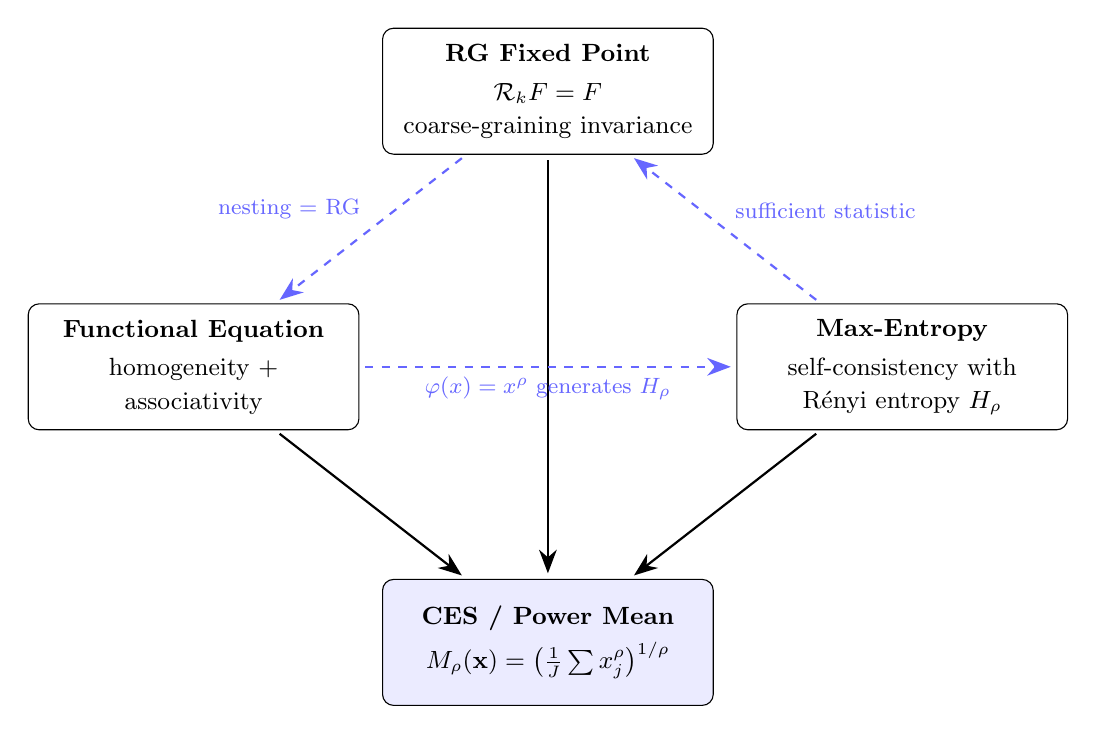
\begin{tikzpicture}[
    box/.style={draw, rounded corners, minimum width=4.2cm, minimum height=1.6cm, align=center, font=\small},
    arr/.style={-{Stealth[length=3mm]}, thick, shorten >=2pt, shorten <=2pt}
]
\node[box] (rg) at (0,3.5) {\textbf{RG Fixed Point}\\[3pt]$\mathcal{R}_k F = F$\\[1pt]coarse-graining invariance};
\node[box] (fe) at (-4.5,0) {\textbf{Functional Equation}\\[3pt]homogeneity +\\[1pt]associativity};
\node[box] (me) at (4.5,0) {\textbf{Max-Entropy}\\[3pt]self-consistency with\\[1pt]R\'enyi entropy $H_\rho$};
\node[box, fill=blue!8] (ces) at (0,-3.5) {\textbf{CES / Power Mean}\\[3pt]$M_\rho(\mathbf{x}) = \left(\frac{1}{J}\sum x_j^\rho\right)^{1/\rho}$};
\draw[arr] (rg) -- (ces);
\draw[arr] (fe) -- (ces);
\draw[arr] (me) -- (ces);
\draw[arr, dashed, blue!60] (rg) -- node[above left, font=\footnotesize] {nesting = RG} (fe);
\draw[arr, dashed, blue!60] (fe) -- node[below, font=\footnotesize] {$\varphi(x) = x^\rho$ generates $H_\rho$} (me);
\draw[arr, dashed, blue!60] (me) -- node[above right, font=\footnotesize] {sufficient statistic} (rg);
\end{tikzpicture}
\caption{Three arguments converge on CES. Solid arrows: each argument independently implies CES. Dashed arrows: the arguments are connected by deeper equivalences. The power function $\varphi(x) = x^\rho$ simultaneously generates the quasi-arithmetic mean (functional equation), the sufficient statistic for R\'enyi entropy (max-entropy), and the scaling exponent preserved under coarse-graining (RG).}
\label{fig:convergence}
\end{figure}

The unifying object is the \emph{power function} $\varphi(x) = x^\rho$. It simultaneously serves as:
\begin{itemize}
\item The \textbf{generator} of the quasi-arithmetic mean (Acz\'el's theorem).
\item The \textbf{sufficient statistic} for R\'enyi entropy: $H_\alpha$ depends on $\mathbf{p}$ only through $\sum p_j^\alpha$.
\item The \textbf{scaling exponent} preserved under renormalization: the $L^\rho$ norm is self-similar.
\end{itemize}
The power function is the unique family with all three properties, and CES is the production function it generates.


%% ============================================================
\section{The $\rho$ Universality Class}\label{sec:universality}
%% ============================================================

\subsection{$\rho$ as a Critical Exponent}

In statistical mechanics, universality classes are labeled by \emph{critical exponents}---numbers that are preserved under renormalization and determine the qualitative behavior of the system near phase transitions. The parameter $\rho$ plays exactly this role for economic aggregation.

\begin{proposition}[$\rho$ is marginal]\label{prop:marginal}
Under the aggregation RG, $\rho$ has scaling dimension zero: $\rho' = \rho + O(\epsilon^2)$ where $\epsilon$ measures the deviation from CES. Non-CES perturbations decay geometrically while $\rho$ is preserved.
\end{proposition}

Different values of $\rho$ define qualitatively different economic regimes:

\begin{center}
\begin{tabular}{lccc}
\toprule
Regime & $\rho$ range & Equilibrium distribution & Economic character \\
\midrule
Strong complements & $\rho < 0$ & Power-law ($q$-exponential, $q < 1$) & Bottleneck-dominated \\
Unit elasticity & $\rho = 0$ & Log-normal (Gibbs-Boltzmann) & Balanced \\
Weak substitutes & $0 < \rho < 1$ & Stretched exponential ($q > 1$) & Abundance-dominated \\
Perfect substitutes & $\rho = 1$ & Degenerate (winner-take-all) & Commodity \\
\bottomrule
\end{tabular}
\end{center}

The critical boundary $\rho = 0$ (Cobb-Douglas) separates complementary from substitutable regimes. At this boundary, the equilibrium distribution is exactly log-normal---the standard Gibbs-Boltzmann distribution of statistical mechanics. Moving away from $\rho = 0$ in either direction ``deforms'' the distribution, generating heavier or lighter tails.

\subsection{Connection to Tsallis Thermodynamics}

The identification $q = \rho$ connects the CES framework to Tsallis non-extensive statistical mechanics \citep{tsallis1988}. Tsallis introduced the deformation parameter $q$ to handle systems with long-range correlations, where the standard Boltzmann-Gibbs framework (which assumes weak correlations and extensivity) breaks down.

In the economic context, the mapping is:
\begin{itemize}
\item $q = 1$ ($\rho = 1$, perfect substitutes): agents are independent, entropy is extensive (Shannon), distributions are exponential. This is the standard competitive equilibrium.
\item $q < 1$ ($\rho < 1$, complements): agents are \emph{positively correlated} through the complementarity of the production function. Entropy is sub-extensive. Distributions are heavy-tailed. Small perturbations to bottleneck inputs have outsized effects on the aggregate.
\item $q > 1$: not economically relevant for production (would imply $\rho > 1$, an increasing-returns CES), but appears in consumption aggregation where goods can be ``super-substitutes.''
\end{itemize}

\begin{proposition}[Tail exponent]\label{prop:tail}
The equilibrium allocation under $F_q = \Phi_{\text{CES}}(q) - T \cdot S_q$ has tail behavior
\begin{equation}\label{eq:tail}
p_j \sim \varepsilon_j^{-1/(1-q)} \quad \text{as } \varepsilon_j \to \infty,
\end{equation}
for $q < 1$. The Pareto exponent is $\zeta = 1/(1-\rho)$, which is the elasticity of substitution $\sigma$.
\end{proposition}

This provides a deep explanation for the ubiquity of power laws in economics \citep{gabaix2009}: they emerge from complementary production ($\rho < 0$) combined with entropy maximization at $T > 0$ (Remark~\ref{rem:T-positive}). The Pareto exponent is not a free parameter---it is determined by the production technology through $\sigma = 1/(1-\rho)$.  More precisely, $\rho$ determines the \emph{shape} of the tail (the exponent $\zeta$), while $T$ determines whether the tail \emph{exists at all} (it vanishes as $T \to 0$).

\subsection{The $\rho$ Phase Diagram}

Combining the universality class with the temperature $T$ yields the complete phase diagram of economic aggregation:

\begin{figure}[h]
\centering
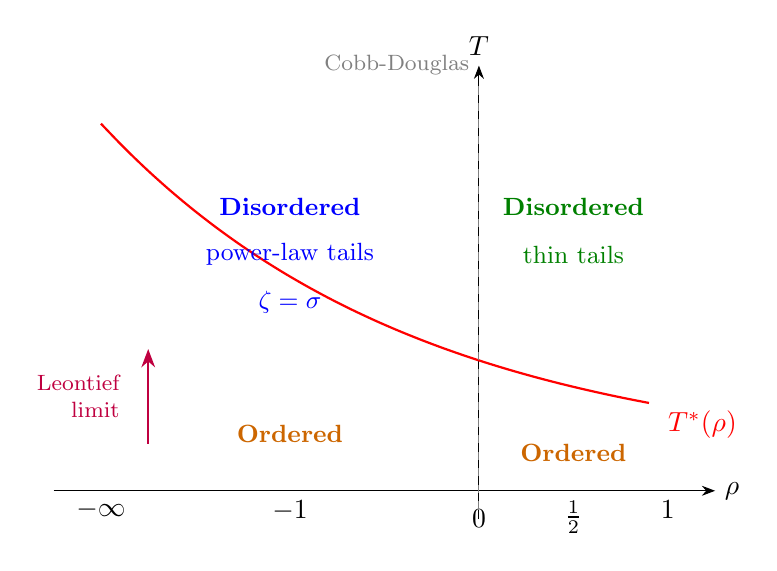
\begin{tikzpicture}[scale=1.2]
% axes
\draw[-{Stealth}] (-4.5,0) -- (2.5,0) node[right] {$\rho$};
\draw[-{Stealth}] (0,-0.3) -- (0,4.5) node[above] {$T$};
% labels
\node[below] at (-4,0) {$-\infty$};
\node[below] at (-2,0) {$-1$};
\node[below] at (0,-0.1) {$0$};
\node[below] at (1,0) {$\frac{1}{2}$};
\node[below] at (2,0) {$1$};
% critical curve
\draw[thick, red] plot[smooth, domain=-4:1.8] (\x, {0.3 + 0.8*exp(-0.3*(\x-1))});
\node[red, right] at (1.9,0.7) {$T^*(\rho)$};
% regions
\node[blue] at (-2, 3) {\small\textbf{Disordered}};
\node[blue] at (-2, 2.5) {\small power-law tails};
\node[blue] at (-2, 2.0) {\small $\zeta = \sigma$};
\node[green!50!black] at (1, 3) {\small\textbf{Disordered}};
\node[green!50!black] at (1, 2.5) {\small thin tails};
\node[orange!80!black] at (-2, 0.6) {\small\textbf{Ordered}};
\node[orange!80!black] at (1, 0.4) {\small\textbf{Ordered}};
% Cobb-Douglas line
\draw[dashed, gray] (0,-0.2) -- (0,4.3);
\node[gray, above left] at (0,4.3) {\footnotesize Cobb-Douglas};
% annotations
\draw[{Stealth}-, thick, purple] (-3.5, 1.5) -- (-3.5, 0.5);
\node[purple, left, font=\footnotesize, align=right] at (-3.7, 1.0) {Leontief\\limit};
\end{tikzpicture}
\caption{Phase diagram of economic aggregation in $(\rho, T)$ space. The critical curve $T^*(\rho)$ separates ordered (low-$T$, efficient) from disordered (high-$T$, noisy) regimes. Below the critical curve, allocations are approximately optimal; above it, entropy dominates. The Cobb-Douglas boundary ($\rho = 0$) separates power-law equilibria (left) from thin-tailed equilibria (right). The tail exponent $\zeta = \sigma = 1/(1-\rho)$ is determined by the universality class.}
\label{fig:phase}
\end{figure}


%% ============================================================
\section{Implications for the $(\rho, T)$ Framework}\label{sec:implications}
%% ============================================================

\subsection{Axiom Reduction}

The $(\rho, T)$ economic free energy framework \citep{smirl2026unified} rests on five axioms. Axiom~A1 states: ``Production at each level is CES.'' \Cref{thm:emergent} shows that A1 can be replaced by two weaker axioms:

\begin{center}
\begin{tabular}{lll}
\toprule
Original & Replacement & Content \\
\midrule
A1: CES production & A1a: Constant returns & Homogeneity of degree 1 \\
 & A1b: Scale consistency & Associative aggregation \\
\bottomrule
\end{tabular}
\end{center}

This is not merely an aesthetic improvement. The original A1 is a parametric assumption about functional form---the kind of assumption that invites the response ``but what if production isn't CES?'' The replacements are structural properties: constant returns is standard in aggregation theory, and scale consistency is the requirement that macro quantities are well-defined (independent of arbitrary partitioning choices). The response ``what if aggregation isn't scale-consistent?'' is much harder to sustain---it amounts to claiming that economic aggregates depend on the analyst's choice of sector boundaries.

\subsection{Why $\rho$ Is the Natural Parameter}

The emergence result explains why $\rho$---rather than $\sigma = 1/(1-\rho)$, or $K = (1-\rho)(J-1)/J$, or any other reparameterization---is the natural parameter of the framework.

\begin{enumerate}
\item \textbf{RG invariance}: $\rho$ is the exponent preserved under coarse-graining. $\sigma$ and $K$ are derived quantities.
\item \textbf{Entropy matching}: $\rho$ equals the R\'enyi order $\alpha$. No other parameterization has this property.
\item \textbf{Universality class label}: $\rho$ determines the equilibrium distribution's tail behavior. $\sigma$ does too (it's a function of $\rho$), but $\rho$ is the primitive object---the power in the power mean.
\item \textbf{Tsallis deformation}: $\rho = q$ in the Tsallis framework. The deformation of thermodynamics is parameterized by $\rho$ directly.
\end{enumerate}

That said, different derived quantities are natural in different contexts. The curvature $K = (1-\rho)(J-1)/J$ is natural for the quadruple-role theorem because it measures the gap between CES and linear aggregation at the symmetric point. The elasticity $\sigma = 1/(1-\rho)$ is natural for demand analysis because it directly gives the percentage response to relative price changes. The emergence result says that $\rho$ is the \emph{fundamental} parameter from which these are derived.

\subsection{The Translog as an Irrelevant Perturbation}

The translog production function \citep{christensen1973} is the standard ``flexible'' alternative to CES:
\begin{equation}\label{eq:translog}
\log F(\mathbf{x}) = \alpha_0 + \sum_j \alpha_j \log x_j + \frac{1}{2}\sum_{j,k} \beta_{jk} \log x_j \log x_k.
\end{equation}
The translog nests Cobb-Douglas ($\beta_{jk} = 0$) but not general CES. From the RG perspective, the translog adds irrelevant operators to the Cobb-Douglas fixed point: the $\beta_{jk}$ terms break scale consistency and vanish under coarse-graining. The translog is not an alternative to CES---it is a transient deviation from CES that exists only at fine scales.

This resolves a long-standing puzzle in production economics: why CES fits aggregate data well despite being ``more restrictive'' than translog. The answer is that the translog's extra flexibility is precisely the kind of flexibility that doesn't survive aggregation. Estimating a translog at the macro level is fitting noise---the irrelevant operators that haven't yet been averaged away.

\subsection{Weighted CES and Asymmetric Inputs}

The emergence theorem (\Cref{thm:emergent}) assumes symmetric inputs. Real economies have heterogeneous input shares. The weighted CES
\begin{equation}\label{eq:weighted_ces}
F_\rho(\mathbf{x}; \mathbf{w}) = \left(\sum_{j=1}^J w_j x_j^\rho\right)^{1/\rho}, \qquad w_j > 0, \quad \sum_j w_j = 1,
\end{equation}
is \emph{not} a fixed point of the symmetric RG---the weights break the symmetry. However, weighted CES is the fixed point of the \emph{weighted} aggregation RG, where blocks have unequal sizes and the RG preserves the relative weights. The emergence result generalizes:

\begin{corollary}[Weighted emergence]\label{cor:weighted}
Let $F: \R_+^J \to \R_+$ be continuous, strictly increasing, homogeneous of degree one, and scale-consistent under the weighted partition $\{B_1, \ldots, B_m\}$ with $w_i = |B_i|/J$. Then $F$ is weighted CES with weights $w_j$ proportional to the atoms of the partition.
\end{corollary}

The weights $w_j$ are \emph{not} preserved under coarse-graining in the same way as $\rho$: they can shift as the partition changes. In RG language, the weights are ``dangerously irrelevant''---irrelevant in the scaling sense but capable of affecting non-universal amplitudes. Economically, this means the input shares can vary across levels of aggregation (sector shares $\neq$ firm shares), but the elasticity of substitution is the same at every level.


%% ============================================================
\section{Empirical Predictions}\label{sec:empirical}
%% ============================================================

The emergence of CES generates five testable predictions that distinguish it from the alternative hypothesis that CES is merely a convenient approximation.

\subsection{Prediction 1: CES Fit Improves with Aggregation}

If CES is the RG fixed point and non-CES deviations are irrelevant operators, then CES should fit progressively better at higher levels of aggregation. Specifically:

\begin{prediction}\label{pred:fit}
Let $R^2_\ell$ denote the $R^2$ of the Kmenta approximation (second-order Taylor expansion of CES) relative to the exact production function at aggregation level $\ell$ (establishment $\to$ firm $\to$ industry $\to$ sector $\to$ economy). Then $R^2_{\ell+1} > R^2_\ell$.
\end{prediction}

\textbf{Data}: US Census of Manufactures (establishment-level) aggregated to progressively coarser industry classifications (6-digit $\to$ 4-digit $\to$ 3-digit $\to$ 2-digit NAICS).

\textbf{Test}: Estimate translog at each level; test whether the $\beta_{jk}$ coefficients shrink toward CES-consistency ($\beta_{jk} \to 0$ for $j \neq k$, $\beta_{jj} \to$ common value).

\subsection{Prediction 2: $\rho$ Is Preserved Across Scales}

\begin{prediction}\label{pred:rho_preserved}
The elasticity of substitution $\sigma$ estimated at different aggregation levels should be approximately constant: $\hat{\sigma}_\ell \approx \hat{\sigma}_{\ell'}$ for all $\ell, \ell'$.
\end{prediction}

This is sharper than Prediction~1. It says not only that CES fits better at higher aggregation, but that the \emph{same} $\rho$ fits at every level. Violations would indicate that the RG flow has not converged, which is informative about the ``RG distance'' between the current scale and the fixed point.

\textbf{Data}: Same as Prediction~1, plus cross-country comparisons using Penn World Table capital-labor substitution estimates at different levels of industry aggregation.

\subsection{Prediction 3: Tail Exponents Match $\sigma$}

\begin{prediction}\label{pred:tails}
In sectors with estimated elasticity of substitution $\hat{\sigma}$, the Pareto tail exponent of the firm size distribution should satisfy $\hat{\zeta} \approx \hat{\sigma}$.
\end{prediction}

This prediction connects the production side ($\rho$) to the distributional side (tail exponent) through the Tsallis equilibrium. It is falsifiable: if firm sizes follow a power law for reasons unrelated to the production technology (e.g., preferential attachment in firm growth), then $\hat{\zeta}$ and $\hat{\sigma}$ will be unrelated.

\textbf{Data}: Bureau of Labor Statistics firm size distributions by 3-digit NAICS, combined with sector-level $\sigma$ estimates from \citet{oberfield2014}.

\subsection{Prediction 4: Translog Coefficients Shrink Under Aggregation}

\begin{prediction}\label{pred:translog}
In a translog regression $\log F = \alpha_0 + \sum \alpha_j \log x_j + \frac{1}{2}\sum \beta_{jk} \log x_j \log x_k + \varepsilon$, the ratio $\|\boldsymbol{\beta}\|_F / \|\boldsymbol{\alpha}\|$ (Frobenius norm of the interaction matrix relative to the first-order coefficients) decreases with aggregation level.
\end{prediction}

This is the direct test of irrelevant operators shrinking under the RG. The translog interaction terms $\beta_{jk}$ are the leading irrelevant operators; they should decrease as $O(1/k^\ell)$ where $k$ is the block size and $\ell$ is the number of RG steps.

\subsection{Prediction 5: Complementary Sectors Have Heavier Tails}

\begin{prediction}\label{pred:heavy_tails}
Cross-sectionally, sectors with lower estimated $\rho$ (higher complementarity) should exhibit heavier-tailed firm size distributions: $\partial \hat{\zeta} / \partial \hat{\rho} > 0$, provided $T > 0$ (information friction is non-negligible).
\end{prediction}

This combines the universality class result (\Cref{prop:tail}) with cross-sectional variation. High-complementarity sectors (construction, healthcare, complex manufacturing) should have more extreme firm-size inequality than low-complementarity sectors (commodity agriculture, basic materials).  The qualification $T > 0$ is essential (Remark~\ref{rem:T-positive}): in a hypothetical perfectly optimized sector ($T \to 0$), complementarity compresses rather than stretches the distribution.  In practice, all real sectors have $T > 0$, so the prediction applies; but heavily planned or regulated sectors (lower effective $T$) may show weaker tail effects than market-driven ones at the same $\rho$.


%% ============================================================
\section{Extensions}\label{sec:extensions}
%% ============================================================

\subsection{Nested CES and the RG Flow}

The hierarchical CES structure used in the $(\rho, T)$ framework---different $\rho$ at each level---corresponds to a \emph{non-trivial RG trajectory}: the system has not converged to a single fixed point but instead traces a path through the space of $\rho$ values as the scale changes.

\begin{definition}[RG $\beta$-function for $\rho$]
The RG flow of $\rho$ under coarse-graining from scale $s$ to scale $s + ds$ is
\begin{equation}\label{eq:beta}
\frac{d\rho}{d\log s} = \beta(\rho),
\end{equation}
where $\beta$ encodes how the effective complementarity changes with scale.
\end{definition}

For the CES fixed points, $\beta(\rho) = 0$---$\rho$ is exactly preserved. But if the micro-level production is not exactly CES, or if different scales have genuinely different production structures (e.g., strong complementarity within firms but substitutability across firms), then $\beta(\rho) \neq 0$ and the effective $\rho$ flows.

The fixed points of $\beta$ are the candidates for ``natural'' values of $\rho$ at the macro level:
\begin{itemize}
\item $\rho = 1$ (perfect substitutes): always a fixed point. Stable from above (no $\rho > 1$ for production).
\item $\rho = 0$ (Cobb-Douglas): a fixed point if the micro distribution of productivities is log-normal (by CLT). Stable under mild conditions.
\item $\rho \to -\infty$ (Leontief): a fixed point. Unstable---any substitutability, however small, pulls $\rho$ away from $-\infty$ under aggregation.
\end{itemize}

The empirical elasticity of substitution for aggregate production ($\sigma \approx 0.6$--$0.8$ in most estimates, implying $\rho \approx -0.25$ to $-0.67$) sits between Cobb-Douglas and Leontief, suggesting that the macro economy has not converged to either fixed point. This is consistent with the ``slow RG'' hypothesis: the economy is still flowing toward $\rho = 0$, but the flow is slow enough that the observed $\rho$ remains negative.

\subsection{CES Emergence and Paper 15 (Endogenous $\rho$)}

Paper 15 in the thesis series \citep{smirl2026rho} shows that $\rho$ is endogenous: it evolves through firm optimization, evolutionary selection (the Price equation), and technological standardization (Wright's Law). The emergence result adds a fourth channel: \emph{aggregation itself} can change the effective $\rho$ through the RG flow.

These four channels operate at different scales:
\begin{center}
\begin{tabular}{lll}
\toprule
Channel & Scale & Direction \\
\midrule
Firm optimization & Within firm & Procyclical ($\rho$ rises in booms) \\
Evolutionary selection & Across firms & Diversity-preserving (Price equation) \\
Wright's Law standardization & Technology & Secular increase ($\rho$ rises over time) \\
Aggregation RG & Cross-scale & Flow toward Cobb-Douglas ($\rho \to 0$) \\
\bottomrule
\end{tabular}
\end{center}

The tension between within-scale dynamics (which can push $\rho$ in either direction) and cross-scale aggregation (which pulls toward $\rho = 0$) creates a rich dynamical system whose equilibrium $\rho$ depends on the relative strength of the channels.

\subsection{Beyond Symmetric CES}

The emergence theorem assumes symmetry (identical treatment of all inputs). Real production functions are asymmetric: capital and labor have different shares, skilled and unskilled workers are not interchangeable, etc. How much of the emergence result survives?

The key distinction is between \emph{share asymmetry} (different $w_j$) and \emph{elasticity asymmetry} (different $\rho$ for different input pairs). \Cref{cor:weighted} shows that share asymmetry is compatible with emergence: weighted CES is the fixed point of the weighted RG. But elasticity asymmetry---different $\rho_{jk}$ for different pairs $(j,k)$---breaks the emergence result. There is no simple fixed point when substitution elasticities vary across input pairs.

However, the RG still operates. Under coarse-graining, the effective elasticity matrix $\rho_{jk}$ is averaged across inputs within each block. If the within-block variation in $\rho_{jk}$ is small relative to the between-block variation, the block-level aggregation is approximately CES with $\rho$ equal to the average within-block elasticity. This is a \emph{local} emergence: CES emerges within homogeneous blocks even when the global structure is non-CES.


%% ============================================================
\section{Conclusion}\label{sec:conclusion}
%% ============================================================

The CES production function is not an assumption. It is a theorem---the unique consequence of constant returns to scale and scale consistency. Three independent lines of argument (renormalization group, functional equations, maximum entropy self-consistency) converge on this conclusion, and their convergence is itself a mathematical fact (\Cref{thm:equivalence}).

The implications ramify through the $(\rho, T)$ framework:
\begin{enumerate}
\item The foundational axiom ``production is CES'' is replaced by two structural properties that any multi-scale economy must satisfy. The framework rests on firmer ground.
\item The parameter $\rho$ is identified as a universality class label---the one feature of the production technology that survives aggregation. This explains why CES works empirically: every other feature of the production function is irrelevant in the RG sense.
\item The matching $\rho = \alpha$ (CES parameter = R\'enyi order) locks the production technology to the entropy measure, generating the Tsallis free energy as the natural thermodynamic potential. Heavy-tailed distributions emerge endogenously from complementary production.
\item The translog and other flexible functional forms are reinterpreted as irrelevant perturbations of the CES fixed point---useful for detecting non-CES features at fine scales, but guaranteed to vanish under aggregation.
\item Five empirical predictions (\Cref{sec:empirical}) distinguish the emergence hypothesis from the alternative that CES is merely a convenient approximation.
\end{enumerate}

In the language of statistical mechanics: CES is to production economics what the Gaussian is to probability theory. Not chosen for convenience. Not assumed for tractability. Inevitable.

\clearpage
\begin{thebibliography}{99}

\bibitem[Acz\'el(1948)]{aczel1948}
Acz\'el, J\'anos. 1948. ``On Mean Values.'' \textit{Bulletin of the American Mathematical Society} 54(4): 392--400.

\bibitem[Arrow et~al.(1961)]{arrow1961}
Arrow, Kenneth J., Hollis B. Chenery, Bagicha S. Minhas, and Robert M. Solow. 1961. ``Capital-Labor Substitution and Economic Efficiency.'' \textit{Review of Economics and Statistics} 43(3): 225--250.

\bibitem[Christensen, Jorgenson, and Lau(1973)]{christensen1973}
Christensen, Laurits R., Dale W. Jorgenson, and Lawrence J. Lau. 1973. ``Transcendental Logarithmic Production Frontiers.'' \textit{Review of Economics and Statistics} 55(1): 28--45.

\bibitem[Gabaix(2009)]{gabaix2009}
Gabaix, Xavier. 2009. ``Power Laws in Economics and Finance.'' \textit{Annual Review of Economics} 1(1): 255--294.

\bibitem[Hardy, Littlewood, and P\'olya(1952)]{hardy1952}
Hardy, G. H., J. E. Littlewood, and G. P\'olya. 1952. \textit{Inequalities}. 2nd ed. Cambridge: Cambridge University Press.

\bibitem[Kolmogorov(1930)]{kolmogorov1930}
Kolmogorov, Andrey N. 1930. ``Sur la Notion de la Moyenne.'' \textit{Atti della Reale Accademia Nazionale dei Lincei. Rendiconti} 12: 388--391.

\bibitem[Nagumo(1930)]{nagumo1930}
Nagumo, Mitio. 1930. ``\"Uber eine Klasse der Mittelwerte.'' \textit{Japanese Journal of Mathematics} 7: 71--79.

\bibitem[Oberfield and Raval(2014)]{oberfield2014}
Oberfield, Ezra, and Devesh Raval. 2014. ``Micro Data and Macro Technology.'' NBER Working Paper No. 20452.

\bibitem[Sato(1967)]{sato1967}
Sato, Kazuo. 1967. ``A Two-Level Constant-Elasticity-of-Substitution Production Function.'' \textit{Review of Economic Studies} 34(2): 201--218.

\bibitem[Smirl(2026a)]{smirl2026unified}
Smirl, Jon. 2026a. ``The $(\rho, T)$ Framework: Five Axioms, One Phase Diagram, and the Deductive Structure of Economic Free Energy.'' Working Paper.

\bibitem[Smirl(2026b)]{smirl2026rho}
Smirl, Jon. 2026b. ``Endogenous Complementarity: The Self-Referential Dynamics of $\rho$.'' Working Paper.

\bibitem[Tsallis(1988)]{tsallis1988}
Tsallis, Constantino. 1988. ``Possible Generalization of Boltzmann-Gibbs Statistics.'' \textit{Journal of Statistical Physics} 52(1--2): 479--487.

\end{thebibliography}

\end{document}
